\subsection{Exercise~3.11}

For every point~$x$ in~$X$ let~$f x$ be the pointwise limit of the sequence~$(f_n x)_n$.
The exercise doesn’t specify if the limit function~$f \colon X \to ℝ$ is required to be continuous.



\subsubsection{Non-continuous limit function}

If we don’t require~$f$ to be continuous, then the given assertion is false.

To see this, we consider a sequence~$(x_n)_n$ in the unit interval~$[0, 1]$ that is strictly decreasing and tends to~$0$.
This entails that all the~$x_n$ are nonzero.
We then let~$f_n$ be the real-valued function on~$[0, 1]$ that goes linearly from~$0$ to~$1$ on the interval~$[0, x_n]$, and is~$1$ on~$[x_n, 1]$.
That is,
\[
	f_n
	\colon
	[0, 1] \to ℝ \,,
	\quad
	x
	\mapsto
	\begin{cases*}
		x / x_n & if~$0 ≤ x ≤ x_n$, \\
		1       & if~$x_n ≤ x ≤ 1$,
	\end{cases*}
\]
see \cref{counterexample for increasing sequence}.
\begin{figure}
	\centering
	\begin{tikzpicture}[scale = 2, xscale = 2]
		% axes
		\draw (-0.025, 0) -- (1.1, 0);
		\draw (0, -0.05) node[below]{$0$} -- (0, 1.1);
		% markers
		\draw (0, 1) ++(0.025, 0)-- ++(-0.05, 0) node[left] {$1$};
		\draw (1, 0) ++(0, +0.05) -- ++(0, -0.1) node[below] {$1$};
		% lines
		\draw[thick] (0, 0) -- (0.3, 1) node[above] {$x_n$} -- (1, 1);
	\end{tikzpicture}
	\caption{The continuous function~$f_n \colon [0, 1] \to X$.}
	\label{counterexample for increasing sequence}
\end{figure}
Each function~$f_n$ is continuous, and the sequence of functions~$(f_n)_n$ is increasing because the sequence of points~$(x_n)_n$ is decreasing.
The sequence~$(f_n)_n$ converges pointwise to the function~$f \colon [0, 1] \to X$ given by
\[
	f x
	=
	\begin{cases*}
		0 & if~$x = 0$, \\
		1 & if~$x > 0$.
	\end{cases*}
\]
The limit function~$f$ is non-continuous, and the convergence of~$(f_n)_n$ to~$f$ is not uniform because for every index~$n$ we have
\[
	\sup_{0 ≤ x ≤ 1} {} \abs{f x - f_n x}
	=
	\sup_{0 < x < x_n} 1 - \frac{x}{x_n}
	=
	1 \,.
\]



\subsubsection{Continuous limit function and increasing sequence}

If we require the limit function~$f$ to again be continuous, then the given assertion is true.

To see this, let~$ε > 0$ be arbitrary.
For every index~$n$ we consider the set
\[
	U_n ≔ \{ x ∈ X \suchthat \abs{f x - f_n x} < ε \} \,.
\]
This set is open since it is the preimage of the open interval~$(-ε, ε)$ under the continuous function~$f - f_n$.
Because the sequence~$(f_n)_n$ is increasing we have
\[
	f x = \sup_{n ≥ 0} f_n x
\]
for every point~$x$ in~$X$, the sets~$U_n$ are given by
\[
	U_n = \{ x ∈ X \suchthat f_n x > f x- ε \}
\]
and the sequence of open sets~$U_0, U_1, U_2, \dotsc$ is therefore increasing.
By assumption, every point of~$X$ is contained in some~$U_n$ for~$n$ sufficiently large, whence the sets~$U_n$ form a filtration of~$X$.

It follows from the compactness of the topological space~$X$ that there exists some index~$N$ with~$X = U_N$ and consequently~$U_n = X$ for every~$n ≥ N$.
Therefore,~$\abs{f x - f_n x} < ε$ for every~$x ∈ X$ and every~$n ≥ N$.



\subsubsection{Non-increasing sequence}

Let us give a counterexample that shows that the assertion becomes wrong if we don’t require the sequence~$(f_n)_n$ to be increasing.

We consider once a strictly increasing sequence~$(x_n)_n$ in~$[0, 1]$.
For every index~$n$ we consider now the function~$f_n \colon [0, 1] \to ℝ$ that is a spike of height~$1$ on the interval~$[x_n, x_{n + 1}]$ with spike at the middle point~$(x_n + x_{n + 1})/2$,  and vanishes otherwise;
see \cref{wandering spike function}.
\begin{figure}
	\centering
	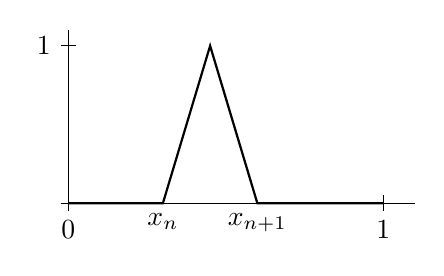
\begin{tikzpicture}[scale = 2, xscale = 2]
		% axes
		\draw (-0.025, 0) -- (1.1, 0);
		\draw (0, -0.05) node[below]{$0$} -- (0, 1.1);
		% markers
		\draw (0, 1) ++(0.025, 0)-- ++(-0.05, 0) node[left] {$1$};
		\draw (1, 0) ++(0, +0.05) -- ++(0, -0.1) node[below] {$1$};
		% lines
		\draw[thick] (0, 0) -- (0.3, 0) node[below] {$x_n$} -- (0.45, 1) -- (0.6, 0) node[below] {$x_{n + 1}$} -- (1, 0);
	\end{tikzpicture}
	\caption{The wandering spike functions~$f_n \colon [0, 1] \to X$.}
	\label{wandering spike function}
\end{figure}
The sequence~$(f_n)_n$ converges pointwise to the zero function as there exists for every point~$x$ in~$[0, 1]$ at most one index~$n$ with~$f_n x ≠ 0$.
The limit function~$f$, which is the zero function, is again continuous.
But the convergence of~$(f_n)_n$ to~$f$ is not uniform since for every index~$n$ we have
\[
	\sup_{0 ≤ x ≤ 1} {} \abs{f x - f_n x}
	=
	\sup_{0 ≤ x ≤ 1} f_n x
	=
	1 \,.
\]
